\documentclass[12pt,letterpaper]{article}

% just for the example
\usepackage{lipsum}
% Set margins to 1.5in
\usepackage[margin=1.5in]{geometry}
\usepackage[toc,page]{appendix}

% for graphics
\usepackage{graphicx}
\graphicspath{{./figures/m3/}}

% for crimson text
\usepackage{crimson}
\usepackage[T1]{fontenc}
\usepackage{url}

% setup parameter indentation
\setlength{\parindent}{0pt}
\setlength{\parskip}{6pt}

% for 1.15 spacing between text
\renewcommand{\baselinestretch}{1.15}

% For defining spacing between headers
\usepackage{titlesec}
% Level 1
\titleformat{\section}
  {\normalfont\fontsize{18}{0}\bfseries}{\thesection}{1em}{}
% Level 2
\titleformat{\subsection}
  {\normalfont\fontsize{14}{0}\bfseries}{\thesection}{1em}{}
% Level 3
\titleformat{\subsubsection}
  {\normalfont\fontsize{12}{0}\bfseries}{\thesection}{1em}{}
% Level 4
\titleformat{\paragraph}
  {\normalfont\fontsize{12}{0}\bfseries\itshape}{\theparagraph}{1em}{}
% Level 5
\titleformat{\subparagraph}
  {\normalfont\fontsize{12}{0}\itshape}{\theparagraph}{1em}{}
% Level 6
\makeatletter
\newcounter{subsubparagraph}[subparagraph]
\renewcommand\thesubsubparagraph{%
  \thesubparagraph.\@arabic\c@subsubparagraph}
\newcommand\subsubparagraph{%
  \@startsection{subsubparagraph}    % counter
    {6}                              % level
    {\parindent}                     % indent
    {12pt} % beforeskip
    {6pt}                           % afterskip
    {\normalfont\fontsize{12}{0}}}
\newcommand\l@subsubparagraph{\@dottedtocline{6}{10em}{5em}}
\newcommand{\subsubparagraphmark}[1]{}
\makeatother
\titlespacing*{\section}{0pt}{12pt}{6pt}
\titlespacing*{\subsection}{0pt}{12pt}{6pt}
\titlespacing*{\subsubsection}{0pt}{12pt}{6pt}
\titlespacing*{\paragraph}{0pt}{12pt}{6pt}
\titlespacing*{\subparagraph}{0pt}{12pt}{6pt}
\titlespacing*{\subsubparagraph}{0pt}{12pt}{6pt}

% Set caption to correct size and location
\usepackage[tableposition=top, figureposition=bottom, font=footnotesize, labelfont=bf]{caption}

% set page number location
\usepackage{fancyhdr}
\fancyhf{} % clear all header and footers
\renewcommand{\headrulewidth}{0pt} % remove the header rule
\rhead{\thepage}
\pagestyle{fancy}

% Overwrite Title
\makeatletter
\renewcommand{\maketitle}{\bgroup
   \begin{center}
   \textbf{{\fontsize{18pt}{20}\selectfont \@title}}\\
   \vspace{10pt}
   {\fontsize{12pt}{0}\selectfont \@author} 
   \end{center}
}
\makeatother

% Used for Tables and Figures
\usepackage{float}

% For using lists
\usepackage{enumitem}

% For using APA Citation format
\usepackage{apacite}

% Custom Quote
\newenvironment{myquote}[1]%
  {\list{}{\leftmargin=#1\rightmargin=#1}\item[]}%
  {\endlist}
  
% Create Abstract 
\renewenvironment{abstract}
{\vspace*{-.5in}\fontsize{12pt}{12}\begin{myquote}{.5in}
\noindent \par{\bfseries \abstractname.}}
{\medskip\noindent
\end{myquote}
}

\begin{document}

% Set Title, Author, and email
\title{Assignment M3}
\author{Snejana Shegheva \\ sshegheva3@gatech.edu}

\maketitle
\thispagestyle{fancy}

\begin{abstract}
Mapping data from one form to another for its ease-of-use is at the core of the \textit{Extract, Transform and Load} process \cite{wiki:etl}. There exist many tools that can accomplish the task of creating and maintaining a data warehouse. However, sometimes it is advantageous to have a custom solution that allows a user to interact with the data directly during some or all of the ETL phases. In this project, we analyze an internal interface of a \textit{transform} task that prepares the data for use in a personalized recommendation system powered by Artificial Intelligence engines. Our main goal is to assess all the weak areas of the existing interface to provide recommendations for alternative models that simplify the user interaction without assuming any pre-existing knowledge of the tool.
\end{abstract}

\subsection*{Brainstorming Plan}
My brainstorming session will be initiated with writing down the core problem, so I can keep it in my sight at all time. I am planning to allocate approximately one hour to session on my blackboard. The choice of a blackboard is driven by the necessity to sketch some ideas rather than plain text only. I intend to generate at least ten ideas, preferably in one session since I am time-boxing it to an hour. Since my task involves an interface I have been interacting with for awhile, I want to constrain myself to come up with a least a few solution that approach the problem in reverse, i.e. is it possible to start with the end-goal and go backwards? Finally, I am not going to erase any ideas during the brainstorming session not matter how unfeasible or ridiculous they may appear. 

\subsection*{Brainstorming Execution}
The brainstorming session resulted in ten ideas (as per plan) and it took about 45-50 minutes to cover my entire blackboard. Figure~\ref{fig::1} shows the artifact of brainstorming where I attempted to sketch the ideas along the text as well. Although the blackboard is pretty big, I have realized that I will be running out of room very soon. Using paper and pen would have been easier, however I tend to come up with more creative ideas using a blackboard.

\begin{figure}[h]
\centering
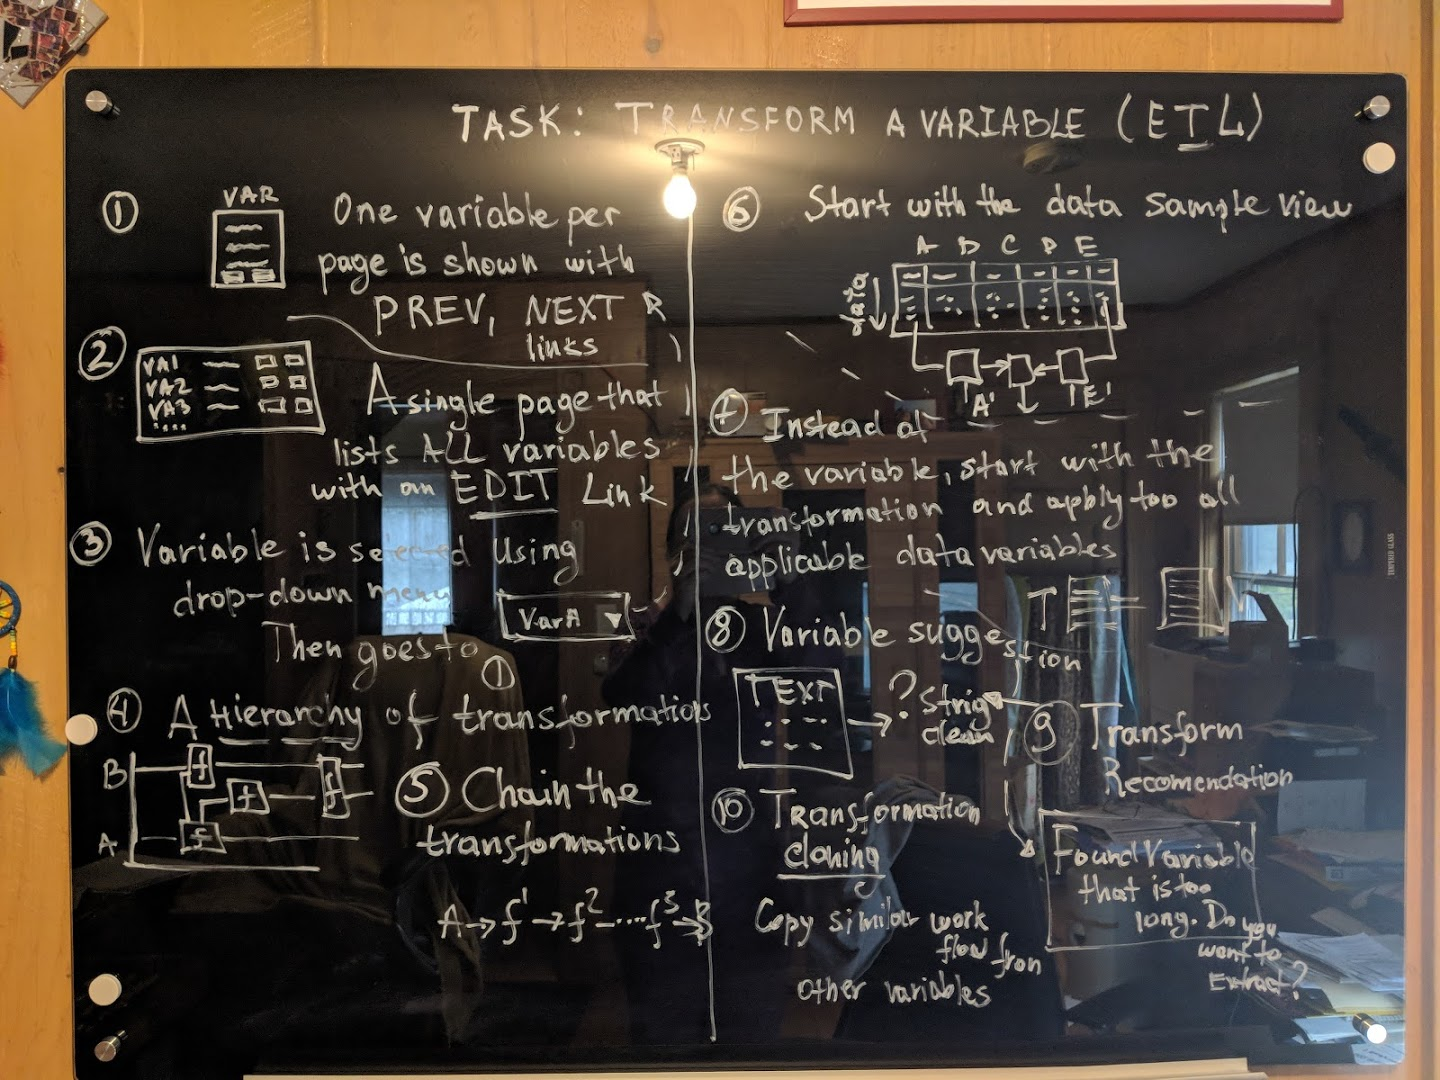
\includegraphics[scale=.3]{figures/m3/brainstorm.jpg}
\caption{Results of the individual brainstorming session for the task of a variable transformation.}
\label{fig::1}
\end{figure}

The scope of the task is to \textit{transform} a variable as part of an ETL process. \underline{Two main directions} that ideas took place are: 1) start with a data field (variable that you wish to change), and find an optimal transformation; 2) start with a view of transformations and match them to the desired variables. Those two directions exemplify a reverse approach towards solving the problem and address the constrain I have set up for myself in the brainstorming rules section.  

Another idea grouping that naturally occurred was using either a single page to show \textit{all} variables, or providing \textit{pagination} interface where user can go to the \textit{next} or \textit{previous} variable. Both have pros and cons, and can be further evaluated using user feedback. 

An interesting idea that appeared is around the concept of recommendations, where the user selects a variable to transform, and instead of browsing through the available toolbox, the user is given a top five for possible transformations functions that are most compatible with the observed variable. I think long term, this idea can prove to be very beneficial, although I can imagine it requires some heavy logic in include the \textit{smartness} in the engine.   



\subsection*{Selection Criteria}
In the process of choosing the top three ideas, I defined the following selection criteria:

\begin{itemize}
    \item The idea should cover the significant count of items from the requirements list. Appendix A enumerates the full set of requirements delivered during the need-finding process.
    \item The idea should be feasible in the short term. After the design is approved, it should not require more than two engineers to implement the approach in two sprints (almost a full month).
    \item The idea should reflect the customer's needs, both internal and external, and should not be designed for a single user. 
\end{itemize}

Based on the selection criteria, these are the top three ideas that we shall move forward with the prototyping:

\begin{itemize}
    \item Idea \#7 as a candidate for the Textual prototype: Start with a list of most common transformations, and map them to one or more data variables.
    \item Idea \#9 as a candidate for the Verbal prototype: Discuss a possible interface where a user is given a recommendation for which transformation function(s) is most compatible with the observed variable.
    \item Idea \#6 as a candidate to the basic form of wire-frames: Guide the user for through the transformation task by keeping a data sample visible at all times.  
\end{itemize}


\subsection*{Prototype 1 - Verbal}

\textit{Imagine that you have an interface through which you can interact with the incoming streams of data. Your goal is to dynamically apply some rules to the received  data. Those rules would transform the current and future data into the desired alternative output. You can treat these transformation rules as simple mathematical functions.}

\textit{The way the system currently works is by iterating through all variables, one at time, giving user an option to edit variable. To find a rule you need to parse through a pile of currently available transformations to find the one most relevant to you. This, of course, could be daunting task if transformations are not organized in any meaningful way.}

\textit{Imagine an alternative way of interacting with a system like that. Let's take as an example a case where you might be looking at a variable that contains a large chunk of text (maybe, transcripts from video lectures). The interface could recommend you a list of most likely transformations, such as:
\begin{itemize}
    \item Remove all punctuation (which could be useful for some subsequent NLP tasks)
    \item Extract keywords (instead of passing the entire text through the pipeline, you might be only interested in the top most representative terms, and entities) 
\end{itemize}
}

\textit{The set you have given is limited to the selected data type. For example, it won't recommend you transformations intended for numerical fields, such as Averaging, Adding/Subtracting, Computing rates, etc. This way your task of transforming can be optimized to your data leading to a more efficient workflow. What do you think?}

\textbf{Evaluation.}
The proposed interface addresses a large chunk of the \textit{functionality} requirements (see Appendix A) by providing means to view, select and apply transformation to incoming streams of data. The \textit{earnability} requirements suggested a need for organization via sorting the current list of transformation. Although, the described prototype does not offer ordering of transformations explicitly, it does so, implicitly via a recommendation engine. Arguably, this could be considered an even better way for organizing a set of functions available in the system. A new interface follows a \textit{discoverability} principle that allows novices and experts to interact with the interface in a more intuitive manner. It addresses portions of the Data Inventory that asks questions on \underline{who are the users?}, \underline{what are their goals, tasks and subtasks?}, \underline{what are their needs?} and \underline{what is the user's context?} 



\subsection*{Prototype 2 - Textual}

A textual prototype: a plaintext description of the idea, how it will work, what its functionality will be, etc. A textual prototype should be sufficiently detailed to get feedback. This is well-suited for many types of design alternatives.

After creating the prototype, evaluate it from the perspective of the requirements you gathered in Assignment M2. Which requirements does it meet? Which requirements does it miss? How well does the prototype mesh with the audience described in your data inventory?

\subsection*{Prototype 3 - Wireframes}

A paper prototype or wireframe: a hand-drawn or simplistic wireframe of the interface you intend to create. It should be thorough enough to get user feedback on its design, but not so detailed that revision would require significant effort; after all, the goal is to get feedback. This is particularly well-suited for a desktop program, tablet app, or web site.

After creating the prototype, evaluate it from the perspective of the requirements you gathered in Assignment M2. Which requirements does it meet? Which requirements does it miss? How well does the prototype mesh with the audience described in your data inventory?

\bibliographystyle{apacite} 
\bibliography{bibtemp}

\newpage
\section*{Appendices}

\appendix

\subsection*{Defining Requirements}

Based on the results from the performed needfinding analysis, we can start describing the desired set of requirements for the interface that supports a data transformation task as part of the ETL process. The recommendations are provided for three areas - functionality, usability and learnability. Our analysis of existing users suggests that we need to cater to both, novices, and experts. The latter group benefits from the speed and efficiency, while the former is comforted with explorative feel of the interface.

\bigskip
\textbf{Functionality} - range of tasks supported for data transformation.

1) The interface must let user \textit{select} a source data intended for modification, \textit{choose} a transformation, \textit{save} the configuration and \textit{apply} the task to the dataset.

2) The interface should give the user a preview of the outcome for selected transformation \textit{before} the task is applied.

3) The interface should allow the user to create/edit/delete transformations, and optionally export it to a human-readable form.

\textbf{Usability} - quality of the available functionality.

1) The interface must support a transformation that is based on multiple sources, for example, combining two fields into one, or performing mathematical operations on them.

2) The interface must provide clear distinction between actions for \textit{saving} a configuration for a transformation, or \textit{applying} the transformation the data.

\textbf{Learnability} - ease and speed for the task of transforming data.

1) The interface should have a toolbox of standard transformations with meaningful names, and built-in tooltip that expands the capabilities of each transformation with examples.

2) The interface should provide clear messaging and notifications on the system's progress. For example, what is the most recent user's request, and what is its status.

3) The interface should allow the user to change the preferences on the order of the available transformations. The current order is alphabetical, and it does not help locate the needed transformation quickly. Options for ordering may include: 

\begin{itemize}
    \item Sort by relevance. Can the interface autodetect the transformations most compatible with the selected data type?
    \item Sort by recency. Show the transformations on top which were accessed last.
    \item Sort by popularity. A user may have a subset of transformations they access the most frequently, so it may be convenient to show a different set of transformations on top without requiring the user to scroll through the large list. 
\end{itemize}

Since the interface described in this project is an internal tool, I have access to the user's feedback that I could use to evaluate the successes of the prototype. For each of the items outlined, I am planning to gathers three data points: 1) priority 2) estimate for implementation 3) feasibility and alignment with the team's goals.

\end{document}
